\documentclass[11pt]{article}

\usepackage[a4paper,left=2.0cm,right=2.0cm,top=2.3cm,bottom=2.3cm]{geometry}
\usepackage{ctex}
\usepackage{amsmath,amssymb,bm}
\usepackage{graphicx}
\usepackage{float}
\usepackage{subcaption}
\usepackage{booktabs}
\usepackage{multirow}
\usepackage{siunitx}
\usepackage[inline]{enumitem}
\usepackage[colorlinks=true,linkcolor=blue,urlcolor=blue]{hyperref}

\setmainfont{Palatino Linotype}
\setCJKmainfont{SimSun}[BoldFont=SimHei,ItalicFont=KaiTi]
\setCJKsansfont{SimHei}
\sisetup{separate-uncertainty=true}
\graphicspath{{ReportFigures/}{analysis_output/}}

% Auto-generated by analysis/boltzmann_analysis.py
\newcommand{\ViMeanUv}{273.4}
\newcommand{\ViStdUv}{21.3}
\newcommand{\CalibrationPointCount}{95}
\newcommand{\GainIntegral}{1.724e+11}
\newcommand{\HeatedTemperatureK}{330.35}
\newcommand{\JohnsonSquareMv}{29.90}
\newcommand{\JohnsonRmsMv}{5.47}
\newcommand{\ResistorOhm}{10000}
\newcommand{\ResistorKOhm}{10.00}
\newcommand{\MeasuredBoltzmann}{1.313e-23}
\newcommand{\BoltzmannRelativeError}{-4.92}
\newcommand{\EffectiveResistance}{9.51e+03}
\newcommand{\EffectiveResistanceKOhm}{9.51}
\newcommand{\CalibrationTable}{%
\begin{tabular}{cccccccc}
\toprule
$f$/kHz & $V_0$/mV & $f$/kHz & $V_0$/mV & $f$/kHz & $V_0$/mV & $f$/kHz & $V_0$/mV\\
\midrule
0.5 & 0.624 & 1 & 3.69 & 1.5 & 6.4 & 2 & 5.52\\
3 & 5.75 & 4 & 12.5 & 5 & 29 & 6 & 58.9\\
7 & 97.6 & 8 & 141 & 9 & 180 & 10 & 216\\
11 & 244 & 12 & 269 & 13 & 289 & 14 & 304\\
15 & 317 & 16 & 326 & 17 & 333 & 18 & 338\\
19 & 334 & 21 & 349 & 22 & 351 & 23 & 352\\
24 & 354 & 25 & 355 & 26 & 356 & 27 & 358\\
28 & 358 & 29 & 358 & 30 & 360 & 31 & 361\\
32 & 362 & 33 & 363 & 34 & 363 & 35 & 364\\
36 & 364 & 37 & 364 & 38 & 365 & 39 & 366\\
40 & 366 & 41 & 366 & 42 & 366 & 43 & 367\\
44 & 367 & 45 & 368 & 46 & 369 & 47 & 369\\
48 & 369 & 49 & 368 & 50 & 367 & 51 & 367\\
52 & 365 & 53 & 366 & 54 & 365 & 55 & 364\\
56 & 364 & 57 & 364 & 58 & 362 & 59 & 360\\
60 & 360 & 61 & 359 & 62 & 358 & 63 & 357\\
64 & 355 & 65 & 354 & 66 & 352 & 67 & 350\\
68 & 349 & 69 & 346 & 70 & 344 & 71 & 342\\
72 & 341 & 73 & 339 & 74 & 336 & 75 & 331\\
76 & 331 & 77 & 329 & 78 & 328 & 79 & 325\\
80 & 322 & 85 & 311 & 90 & 299 & 95 & 285\\
100 & 274 & 105 & 266 & 110 & 253 & 115 & 241\\
120 & 229 & 125 & 220 & 130 & 209 & 135 & 198\\
140 & 188 & 145 & 177 & 150 & 165 &  & \\
\bottomrule
\end{tabular}
}
\newcommand{\NoiseGroupTable}{%
\begin{tabular}{lrrrr}\toprule
分组 & 读数个数 & 平均 RMS/mV & 标准差/mV & 均方/mV$^2$\\\midrule
常温接入电阻 & 14 & 7.739 & 0.222 & 59.94\\
加热短路本底 & 9 & 3.211 & 0.097 & 10.32\\
加热接入电阻 & 9 & 6.295 & 0.816 & 40.22\\
\bottomrule\end{tabular}
}


\newcommand{\experiName}{电阻热噪声测量玻尔兹曼常数}
\newcommand{\supervisor}{王佳怡}
\newcommand{\name}{邓思豪}
\newcommand{\studentNum}{2023K8009909008}
\newcommand{\class}{3}
\newcommand{\group}{01}
\newcommand{\seat}{5}
\newcommand{\dateYear}{2026}
\newcommand{\dateMonth}{1}
\newcommand{\dateDay}{7}
\newcommand{\room}{西实204}
\newcommand{\others}{$\square$}

\begin{document}

\begin{center}
    \LARGE\bfseries 中国科学院大学物理实验报告
\end{center}

\begin{center}
    \noindent 实验名称\underline{\makebox[23em][c]{\experiName}}
    指导教师\underline{\makebox[7em][c]{\supervisor}}\\
    姓名\underline{\makebox[6em][c]{\name}}
    学号\underline{\makebox[11em][c]{\studentNum}}
    分班分组及座号\underline{\makebox[6em][c]{\class-\group-\seat 号}}\\
    实验日期\underline{\makebox[3em][c]{\dateYear}}年
    \underline{\makebox[2em][c]{\dateMonth}}月
    \underline{\makebox[3em][c]{\dateDay}}日
    实验地点\underline{\makebox[7em][c]{\room}}
    调课/补课\underline{\makebox[3em][c]{\others\ 否}}
    成绩评定\underline{\hspace{4em}}\\[-0.3em]
    \rule[8pt]{17cm}{0.2em}
\end{center}

\section{实验目的}

\begin{enumerate}
    \item 了解热力学和统计物理中玻尔兹曼常数的物理意义，认识热噪声作为微观热运动宏观表现的实验价值。
    \item 熟悉前置放大器、带通滤波器、函数发生器、示波器和恒温加热台等电子学仪器的基本使用方法。
    \item 通过标准正弦信号校准测量系统的频率响应，获得有效增益曲线 $g(f)$ 和增益积分 $G$。
    \item 测量电阻 Johnson 噪声的有效值，扣除测量系统本底噪声，理解 $V_J^2\propto T$ 的热噪声规律。
    \item 利用已知阻值 $R=\SI{\ResistorKOhm}{k\ohm}$ 计算玻尔兹曼常数，并从带宽、本底、温度和寄生参数等方面分析偏差来源。
\end{enumerate}

\section{实验仪器与用具}

\begin{itemize}
    \item 函数发生器：产生已知频率和幅值的正弦信号，用于校准整套放大与滤波链路的频率响应。
    \item 衰减器：将函数发生器输出衰减到毫伏或亚毫伏量级，使校准输入接近噪声测量时的微弱信号水平。
    \item SRS 差分前置放大器：对微弱电压进行低噪声放大，校准时使用单端输入，噪声测量时使用 $A-B$ 差分输入。
    \item 带通滤波器：限制测量带宽，压低低频漂移和高频干扰，使积分带宽可由校准曲线确定。
    \item 数字示波器：读取输出信号的 RMS 有效值，并记录不同频率或不同连接方式下的波形。
    \item 待测电阻、短路夹具与屏蔽盒：提供热噪声源，并通过短路读数测量系统本底噪声。
    \item 恒温加热台：改变电阻温度。本次加热测量采用照片读数 \SI{57.2}{\degreeCelsius}。
\end{itemize}

\section{实验原理}

\subsection{Johnson 噪声与 Nyquist 公式}

处于热平衡的电阻中，载流子由于热运动不断发生无规则涨落，即使没有外加电流，电阻两端也会出现随机起伏的电压。Nyquist 从热力学第二定律和能量均分定理出发，给出单位频带内电阻热噪声均方电压
\begin{equation}
    \mathrm d V_J^2=4k_BTR\,\mathrm df ,
\end{equation}
其中 $k_B$ 为玻尔兹曼常数，$T$ 为电阻热力学温度，$R$ 为电阻值。若理想测量系统在频带 $\Delta f$ 内具有平坦响应，则有
\begin{equation}
    V_J^2=4k_BTR\Delta f .
\end{equation}

实际实验中，前置放大器、滤波器和示波器构成的链路具有随频率变化的增益。用 RMS 幅值为 $V_i$ 的标准正弦信号校准，在频率 $f$ 处测得输出 RMS 幅值 $V_0(f)$，定义
\begin{equation}
    g(f)=\frac{V_0(f)}{V_i}.
\end{equation}
若考虑导线与接触处的等效电容 $C$，电阻与电容并联造成的高频修正为
\begin{equation}
    R_f=\frac{R}{1+(2\pi fRC)^2}.
\end{equation}
总增益积分为
\begin{equation}
    G=\int_0^\infty \frac{|g(f)|^2}{1+(2\pi fRC)^2}\,\mathrm df.
    \label{eq:gain_integral}
\end{equation}
于是示波器端测得并扣除系统本底后的均方电压满足
\begin{equation}
    V_J^2=4k_BTRG.
    \label{eq:johnson}
\end{equation}
本实验资料中未给出接触电容 $C$，数据处理取 $C=0$，即将式 \eqref{eq:gain_integral} 化为 $G=\int |g(f)|^2\mathrm df$。该近似会忽略高频端的并联电容衰减，是结果讨论中的主要系统误差来源之一。

\subsection{短路本底扣除}

测量系统自身也会产生噪声。将待测电阻短路后，示波器读得的 RMS 值记为 $V_s$；接入电阻后读得 $V_n$。在两组噪声统计独立的近似下，电阻热噪声贡献写为
\begin{equation}
    V_J^2=\langle V_n^2\rangle-\langle V_s^2\rangle .
\end{equation}
由于示波器的瞬时 RMS 读数不断波动，实验需要对多张截图或多次读数取均方平均，而不是直接对 RMS 值作线性相减。

\section{实验内容}

\begin{enumerate}
    \item 按校准电路连接函数发生器、衰减器、前置放大器、带通滤波器和示波器。接线前将前置放大器输入置于 GND 档，确认各仪器供电和接地正常。
    \item 使用约毫伏量级的标准正弦输入，在不改变输入幅值和放大器设置的前提下改变频率，记录输出 RMS 值 $V_0(f)$。扫描 PDF 记录了 \SIrange{0.5}{80}{kHz} 的数据，\texttt{V\_i.xlsx} 记录了 \SIrange{85}{150}{kHz} 的后续数据。
    \item 按噪声测量电路连接待测电阻，使两根输入线尽量短且相互缠绕，并将前置放大器改为 $A-B$ 差分输入。保持校准阶段的增益、滤波和示波器设置不变。
    \item 在常温接入电阻时记录多张示波器截图，作为稳定性对照。
    \item 将电阻置于恒温加热台上升温，分别记录加热短路本底和加热接入电阻时的输出 RMS 值。加热台照片显示实际温度约为 \SI{57.2}{\degreeCelsius}。
    \item 用校准曲线计算 $G$，再由加热接入读数扣除加热短路本底，得到 $V_J^2$。待测电阻取 $R=\SI{\ResistorKOhm}{k\ohm}$，代入 Johnson--Nyquist 公式计算 $k_B$。
\end{enumerate}

\begin{figure}[H]
    \centering
    \begin{subfigure}{0.31\textwidth}
        \centering
        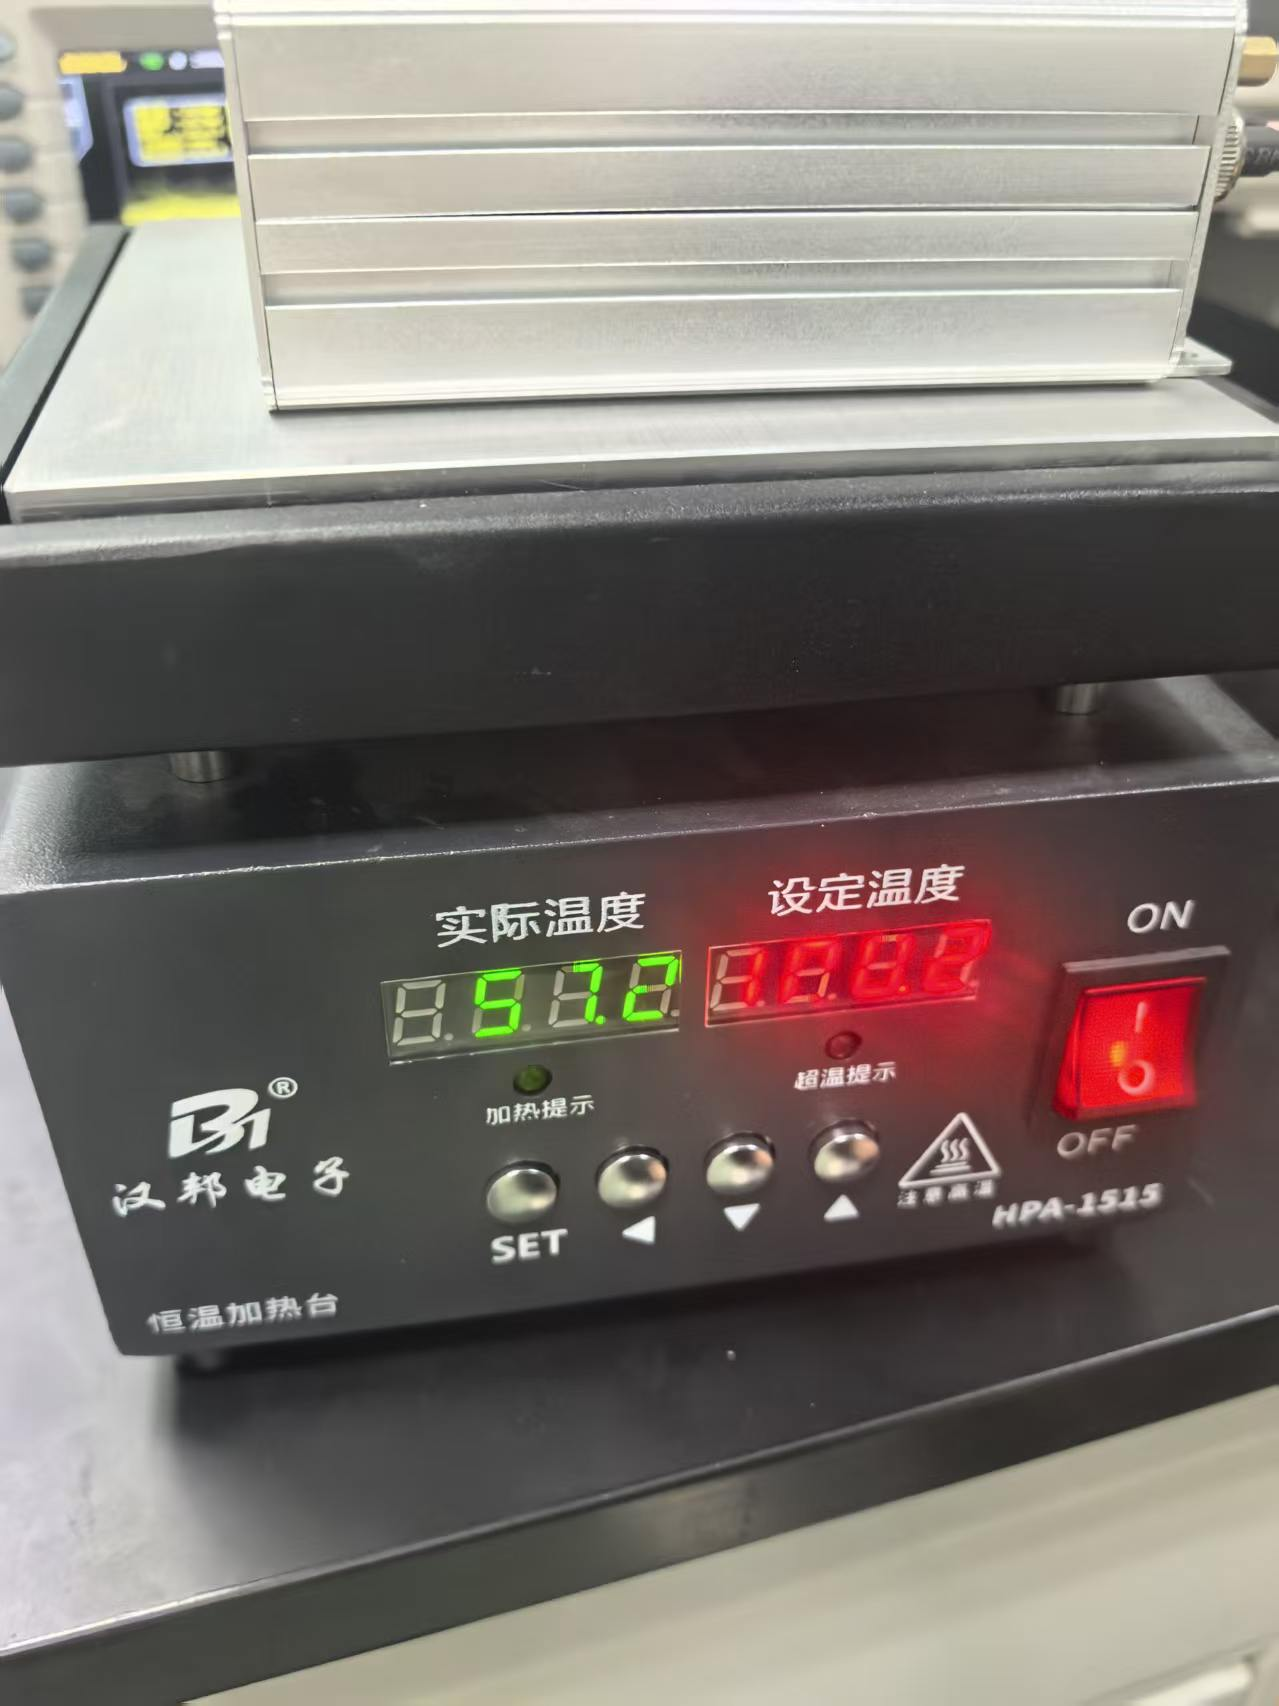
\includegraphics[width=\textwidth]{heater_temperature.jpg}
        \caption{加热台温度}
    \end{subfigure}
    \begin{subfigure}{0.31\textwidth}
        \centering
        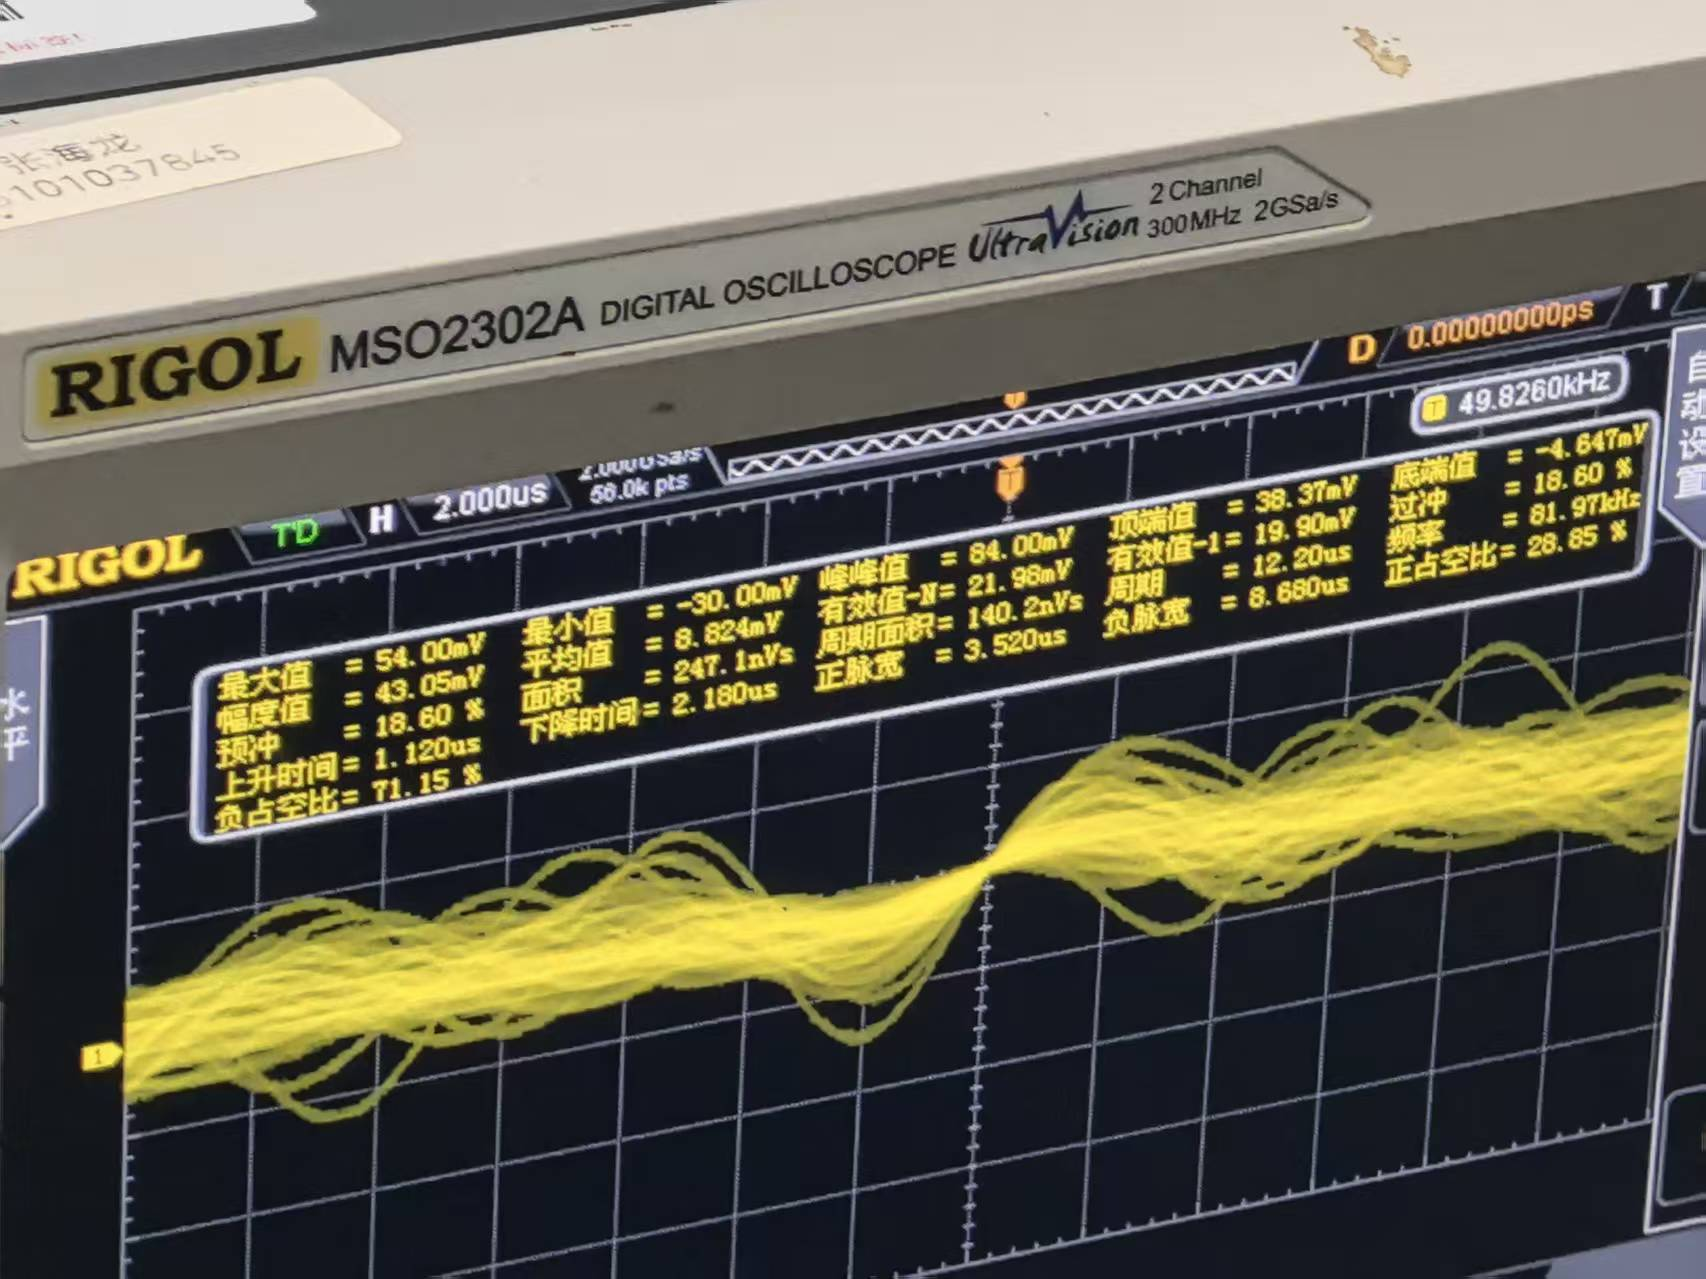
\includegraphics[width=\textwidth]{heated_short_example.jpg}
        \caption{加热短路本底}
    \end{subfigure}
    \begin{subfigure}{0.31\textwidth}
        \centering
        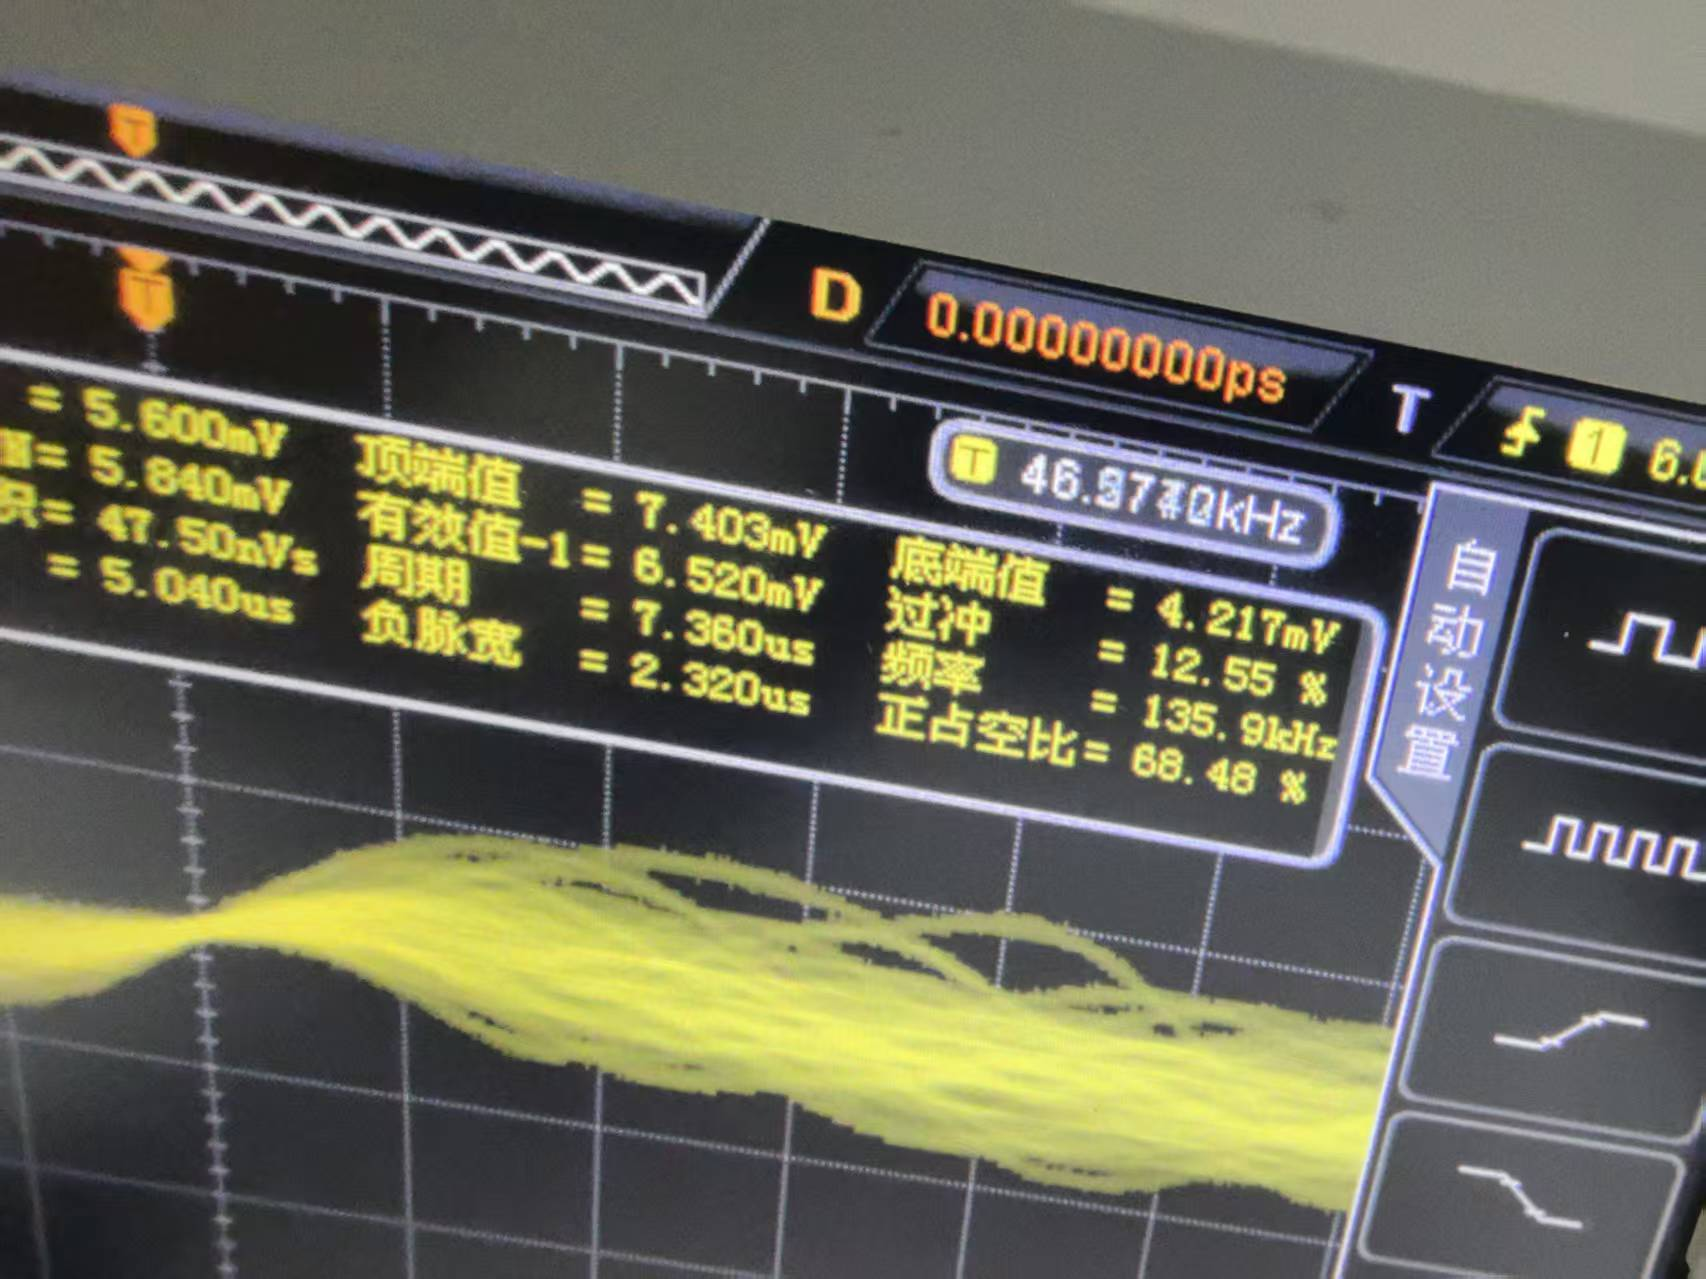
\includegraphics[width=\textwidth]{heated_resistor_example.jpg}
        \caption{加热接入电阻}
    \end{subfigure}
    \caption{实验记录中的代表性照片}
\end{figure}

\section{实验数据处理}

\subsection{校准数据与增益积分}

扫描 PDF 第一页顶部给出十次校准输入 RMS 读数，平均为
\begin{equation}
    \bar V_i=\SI{\ViMeanUv}{\micro V},\qquad s_{V_i}=\SI{\ViStdUv}{\micro V}.
\end{equation}
本报告将其作为整个校准过程中输入幅值的估计。扫描 PDF 的 \SIrange{0.5}{80}{kHz} 数据与 \texttt{V\_i.xlsx} 的 \SIrange{85}{150}{kHz} 数据合并后共有 \CalibrationPointCount 个频率点，见表 \ref{tab:calibration}。

\begin{table}[H]
    \centering
    \caption{校准曲线原始数据。85 kHz 及以上数据来自 \texttt{V\_i.xlsx}。}
    \label{tab:calibration}
    \resizebox{\textwidth}{!}{\CalibrationTable}
\end{table}

由 $g(f)=V_0/\bar V_i$ 得到的有效增益曲线见图 \ref{fig:gain}。曲线在约 \SIrange{35}{50}{kHz} 附近达到平台，低频端受带通滤波器下截止频率影响快速衰减，高频端在 \SI{80}{kHz} 后逐渐下降。采用梯形积分并取 $C=0$ 得到
\begin{equation}
    G=\int |g(f)|^2\,\mathrm df
    = \SI{\GainIntegral}{Hz}.
\end{equation}

\begin{figure}[H]
    \centering
    \begin{subfigure}{0.48\textwidth}
        \centering
        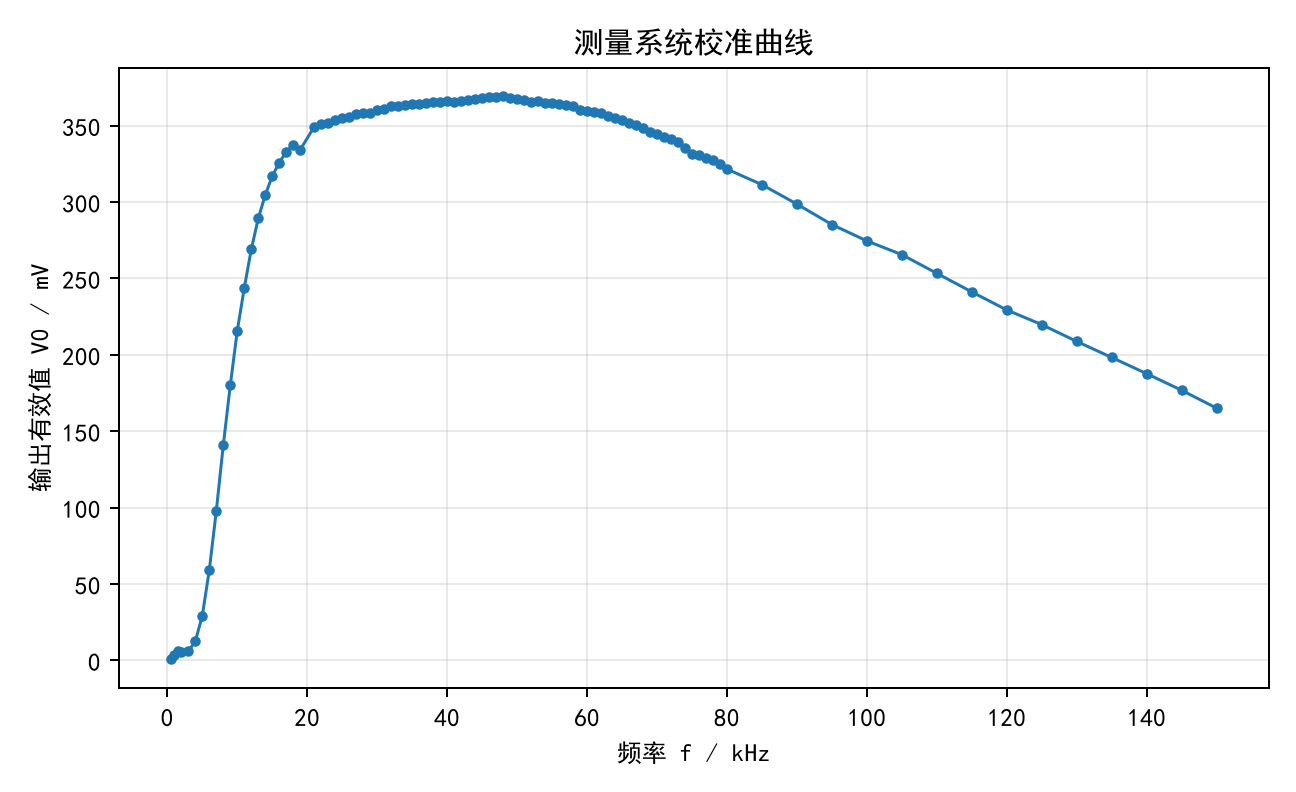
\includegraphics[width=\textwidth]{calibration_curve.png}
        \caption{输出 RMS 随频率变化}
    \end{subfigure}
    \begin{subfigure}{0.48\textwidth}
        \centering
        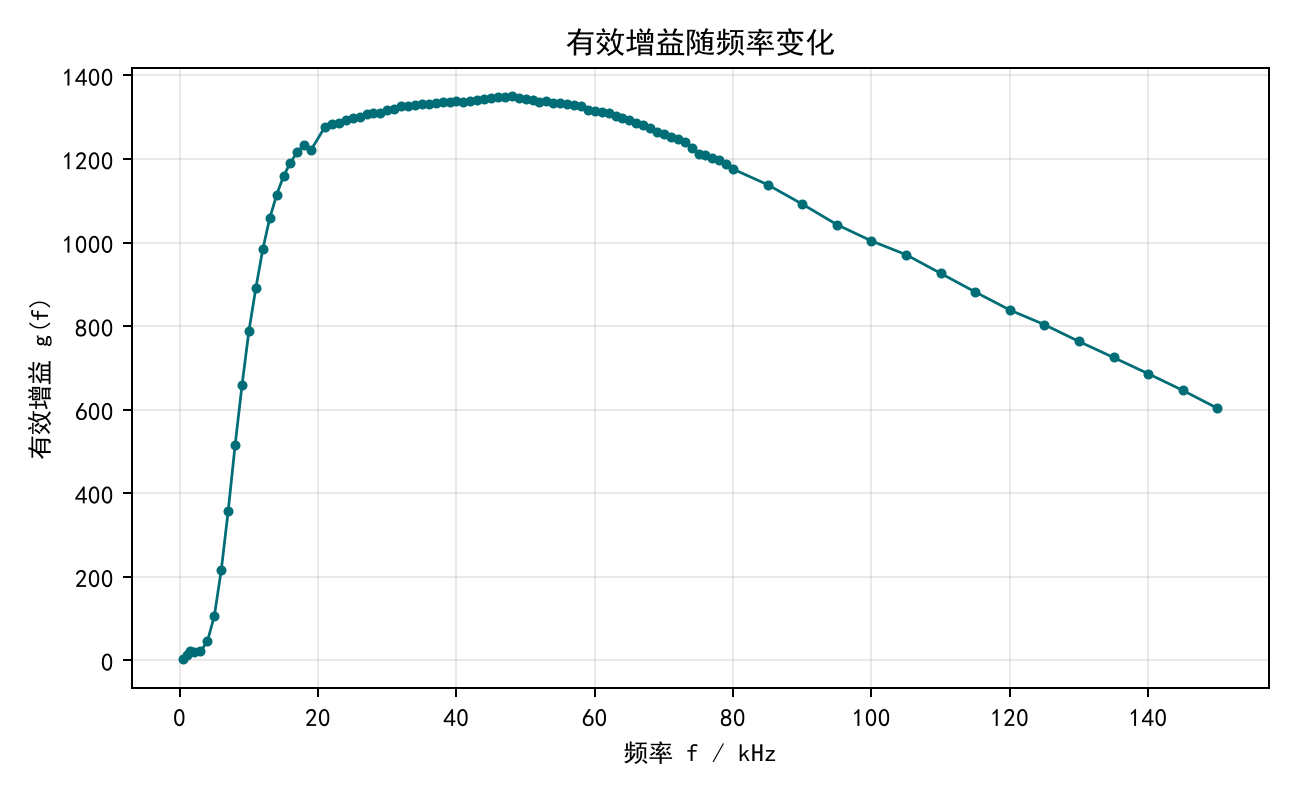
\includegraphics[width=\textwidth]{gain_curve.png}
        \caption{有效增益 $g(f)$}
    \end{subfigure}
    \caption{测量系统的频率响应校准}
    \label{fig:gain}
\end{figure}

\begin{figure}[H]
    \centering
    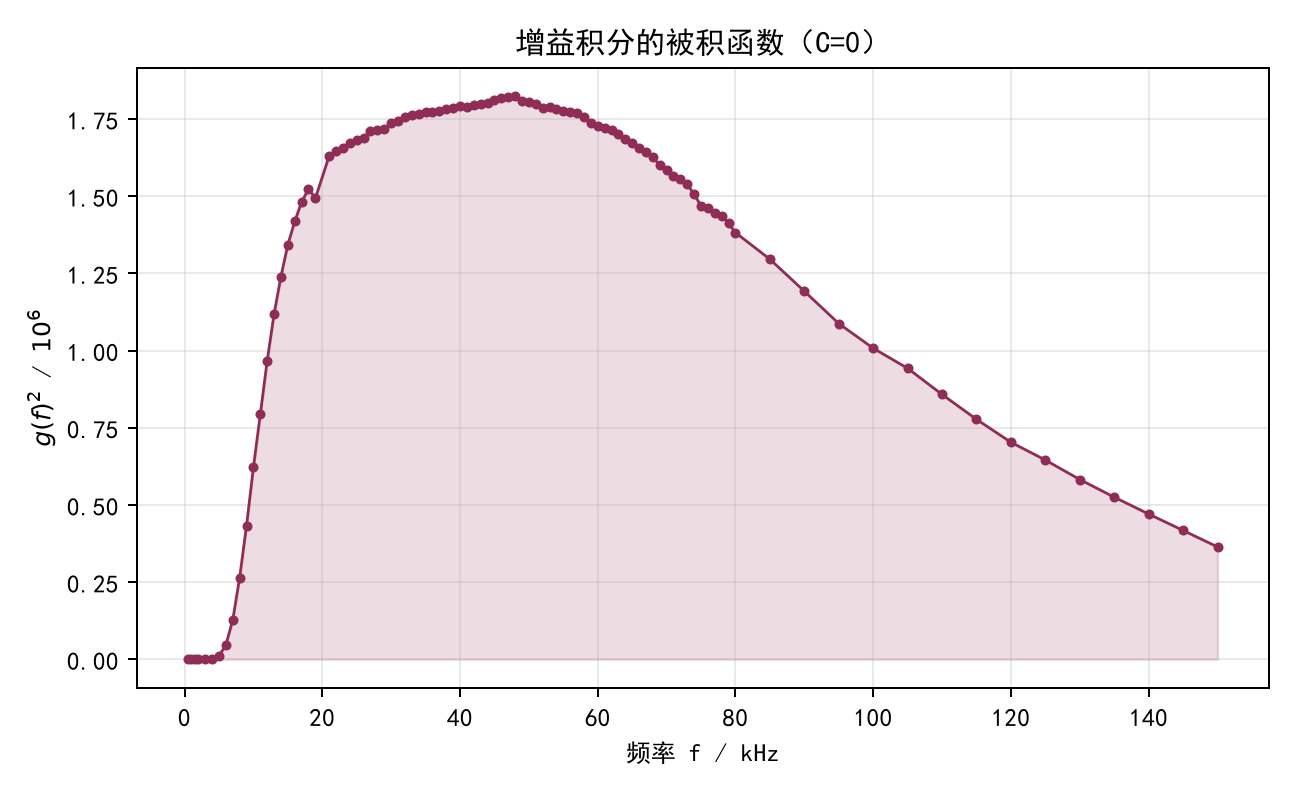
\includegraphics[width=0.72\textwidth]{gain_integrand.png}
    \caption{增益积分被积函数。由于缺少接触电容数据，本图采用 $C=0$。}
\end{figure}

\subsection{噪声读数与本底扣除}

从示波器照片中读取 RMS 有效值并按分组统计，结果见表 \ref{tab:noise}。常温接入电阻数据用于观察系统读数的波动水平；用于最终自洽计算的是同一加热状态下的短路本底和接入电阻两组数据。

\begin{table}[H]
    \centering
    \caption{示波器 RMS 读数分组统计}
    \label{tab:noise}
    \NoiseGroupTable
\end{table}

\begin{figure}[H]
    \centering
    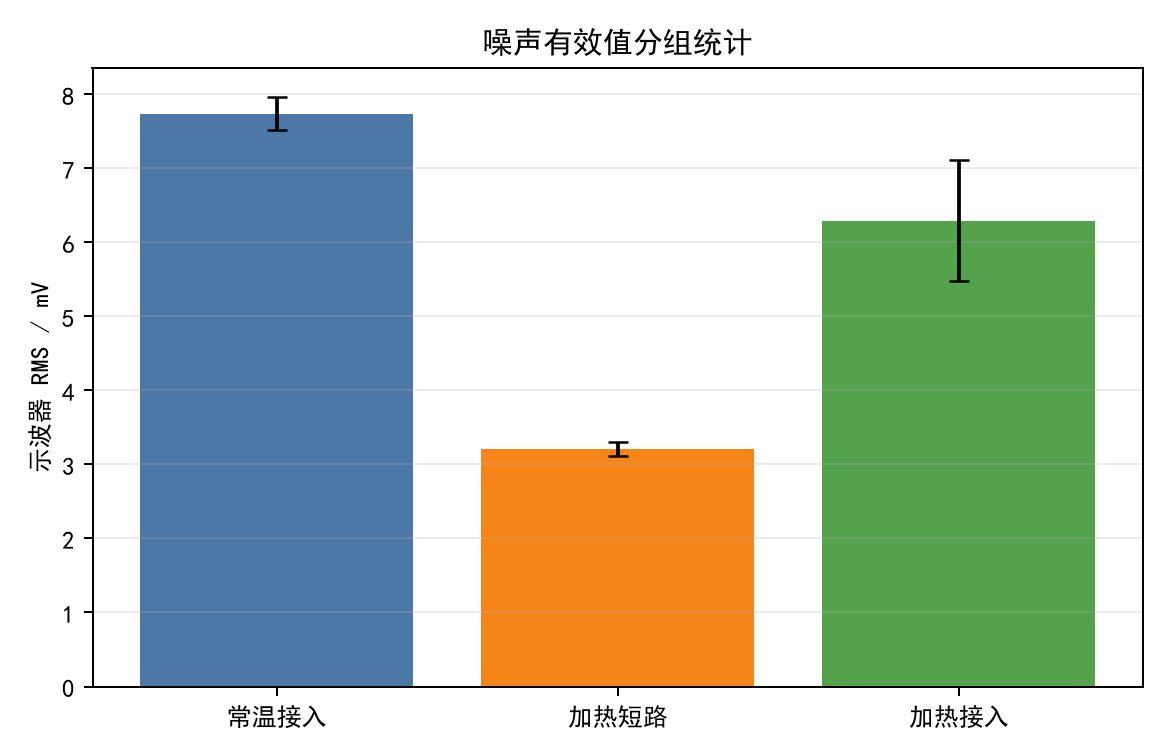
\includegraphics[width=0.68\textwidth]{noise_groups.png}
    \caption{常温、加热短路和加热接入电阻三组 RMS 读数比较}
\end{figure}

加热状态下实际温度取照片读数
\begin{equation}
    T=\SI{57.2}{\degreeCelsius}+\SI{273.15}{K}=\SI{\HeatedTemperatureK}{K}.
\end{equation}
按均方扣除本底，
\begin{equation}
    V_J^2=\langle V_n^2\rangle-\langle V_s^2\rangle
    =\SI{\JohnsonSquareMv}{mV^2},
\end{equation}
对应输出端噪声 RMS 为
\begin{equation}
    V_J=\SI{\JohnsonRmsMv}{mV}.
\end{equation}

\subsection{玻尔兹曼常数计算}

待测电阻取实验记录值
\begin{equation}
    R=\SI{\ResistorOhm}{\ohm}=\SI{\ResistorKOhm}{k\ohm}.
\end{equation}
由式 \eqref{eq:johnson} 得
\begin{equation}
    k_B=\frac{V_J^2}{4TRG}.
\end{equation}
代入 $V_J^2=\SI{\JohnsonSquareMv}{mV^2}$、$T=\SI{\HeatedTemperatureK}{K}$、$R=\SI{\ResistorKOhm}{k\ohm}$ 和 $G=\SI{\GainIntegral}{Hz}$，得到
\begin{equation}
    k_B^{(\mathrm{exp})}
    =\SI{\MeasuredBoltzmann}{J.K^{-1}}.
\end{equation}
与 CODATA 精确值
\begin{equation}
    k_B^{(0)}=\SI{1.380649e-23}{J.K^{-1}}
\end{equation}
相比，相对偏差为
\begin{equation}
    \frac{k_B^{(\mathrm{exp})}-k_B^{(0)}}{k_B^{(0)}}\times 100\%
    =\SI{\BoltzmannRelativeError}{\percent}.
\end{equation}
若反过来使用标准 $k_B$ 检查本次数据的自洽性，可得到等效电阻
\begin{equation}
    R_{\mathrm{eff}}
    =\frac{V_J^2}{4k_B^{(0)}TG}
    \approx \SI{\EffectiveResistanceKOhm}{k\ohm}.
\end{equation}
该值与标称 \SI{\ResistorKOhm}{k\ohm} 接近，说明校准积分、温度和噪声扣本底的总体量级是合理的；两者相差约 $5\%$，也与上式给出的 $k_B$ 偏差方向一致。

\subsection{数据背后的物理分析}

校准曲线的形状直接反映了测量链路的有效带宽。低频端 $V_0$ 很小，是因为带通滤波器和前置放大器的低频滚降抑制了漂移、工频及 $1/f$ 噪声；中频区增益进入平台，说明这一区间的噪声功率会较充分地被放大并进入示波器 RMS 读数；高频端从约 \SI{80}{kHz} 后下降，则来自滤波器上截止频率、放大器带宽以及连线寄生电容的共同作用。因此本实验不能简单取一个几何带宽 $\Delta f$，而必须对 $g(f)^2$ 积分。热噪声功率对频率近似均匀分布，测量系统却只“看见”被增益函数加权后的那部分频谱，$G$ 正是这个加权带宽。

本底扣除也有清楚的物理意义。加热短路时没有待测电阻两端的 Johnson 电压差，但放大器输入噪声、滤波器噪声、示波器量化噪声和环境电磁串扰仍会保留在输出端。接入电阻后的 RMS 读数包含热噪声和这些本底噪声的叠加。独立随机噪声的相位无固定关系，时间平均交叉项趋近于零，所以应在均方意义下相减。若直接相减 RMS，等价于把随机噪声当作同相确定信号，会系统性低估热噪声。

温度升高会线性提高 $V_J^2$，因此加热测量能放大相对于仪器本底的热噪声贡献。不过加热台显示的是台面或外壳附近温度，电阻本体温度还取决于热接触和稳定时间。若电阻实际温度低于读数，则分母 $T$ 被高估，计算出的 $k_B$ 会偏小。本次结果比标准值低约 $4.92\%$，这一偏差方向与“实际电阻温度略低于显示温度”以及“忽略高频寄生电容导致 $G$ 偏大”两种机制都相容。

\subsection{误差分析}

\begin{enumerate}
    \item 校准输入 $V_i$ 的十次读数标准差约为 \SI{\ViStdUv}{\micro V}，相对波动不可忽略。由于 $g(f)=V_0/V_i$，$G$ 与 $1/V_i^2$ 成正比；若 $V_i$ 被低估，则 $G$ 偏大，最终 $k_B=V_J^2/(4TRG)$ 偏小。
    \item 示波器 RMS 读数来自随机噪声波形，短时间内波动明显。数据处理中使用均方平均而非线性平均相减，可以避免低估本底贡献，但截图数量仍限制了统计精度。尤其是加热接入组标准差较大，说明噪声包络仍未完全平均。
    \item 接触电容 $C$ 未测量，本报告取 $C=0$。真实电路中 $RC$ 并联会压低高频贡献，若忽略该项，可能高估高频端对 $G$ 的贡献，从而使计算得到的 $k_B$ 偏小。
    \item 加热台读数是外部温度，待测电阻达到热平衡需要时间。若电阻实际温度低于 \SI{57.2}{\degreeCelsius}，则计算时分母 $T$ 偏大，$k_B$ 也会偏小。
    \item 电阻按 \SI{\ResistorKOhm}{k\ohm} 处理，若实际阻值存在容差或加热后阻值漂移，也会直接等比例影响 $k_B$。金属膜电阻的温度系数虽小，但在几十摄氏度温升下仍可能贡献可见的系统误差。
    \item 噪声测量要求校准和正式测量的前置放大器、滤波器、示波器耦合方式与带宽限制完全一致。任一开关或连线位置改变都会改变 $g(f)$，使先前得到的 $G$ 不再适用。
\end{enumerate}

\section{思考题}

\begin{enumerate}
    \item 为什么校准频率范围不应无限扩大？\\
    校准频率范围应覆盖测量链路真正会通过热噪声的主要通带，而不是越宽越好。Johnson 噪声本身在经典近似下近似为白噪声，单位频带内的噪声功率几乎相同；但是实验测到的是经过前置放大器、滤波器、导线和示波器共同加权后的噪声。因此真正进入结果的是 $\int g^2(f)\,\mathrm df$，而不是人为设定的频率上限。

    过低频处，前置放大器的漂移、工频串扰和 $1/f$ 噪声会更突出，且带通滤波器本来就会压低响应；过高频处，示波器带宽、前置放大器上截止频率、同轴线和接触电容都会使信号衰减。若继续向外扩展频率，新增数据点往往信噪比较差，读数不稳定，反而会把非理想仪器响应误当作热噪声带宽的一部分。本实验校准到 \SI{150}{kHz} 已覆盖主要通带和高频下降段；更有价值的是在上升沿和下降沿加密取点，而不是盲目扩大到更高频率。

    为了测量得更精准，取点密度也应跟随 $g(f)$ 的变化快慢来安排。在低频上升沿和高频滚降区，$g(f)$ 对频率变化很敏感，少量漏点就会明显影响梯形积分，所以应密集取点；在中频平台区，增益变化慢，可以适当稀疏。更进一步，可以先粗扫得到通带范围，再在 $g(f)^2$ 变化最大的区间补点，因为积分权重实际来自 $g^2(f)$ 而不是 $g(f)$ 本身。

    本实验扫描 PDF 中低频到中频已有较密集数据，\texttt{V\_i.xlsx} 补充了 \SIrange{85}{150}{kHz} 的高频下降段，这是必要的；若要进一步提高积分精度，优先补 \SIrange{75}{110}{kHz} 附近的高频滚降段，而不是平台区。这样能更准确估计被积函数尾部面积，从而减小 $G$ 的系统误差。

    \item 示波器的 bandwidth limit 是否可以使用？\\
    可以使用，但前提是校准和正式噪声测量必须保持完全相同的 bandwidth limit 设置。示波器的 bandwidth limit 本质上是在示波器输入端又加入一个低通限制，它会改变测量系统的总频率响应。如果校准时打开，$g(f)$ 已经包含了这个限制，那么之后噪声测量也打开时，计算出的 $G$ 仍然自洽。

    不能接受的是校准和测量设置不一致。例如校准时关闭 bandwidth limit，而噪声测量时打开，则实际噪声带宽小于校准得到的 $G$，计算 $k_B=V_J^2/(4TRG)$ 时会使用过大的 $G$，使 $k_B$ 偏小。反之，校准时打开而测量时关闭，会引入额外高频噪声，使结果偏大或更受环境干扰影响。因此 bandwidth limit 本身不是问题，真正的问题是它是否被纳入校准链路。

    \item 示波器测量使用 AC 模式，若改用 DC 会怎样？\\
    AC 模式会滤去直流偏置和很低频的慢漂移，更适合测量围绕零均值涨落的噪声。Johnson 噪声的理论公式描述的是电压涨落的均方值，而不是某个直流电压，因此去除直流偏置是合理的。若改用 DC 模式，前置放大器输出的零点漂移、热电势、仪器 offset 以及外界慢变化干扰都会进入 RMS 读数，使 RMS 不再只代表随机噪声强度。

    需要注意的是，AC 耦合本身也会改变低频响应，相当于在测量链路中加入一个高通环节。因此 AC/DC 的选择没有绝对对错，关键仍是校准与噪声测量必须一致。本实验若校准时使用 AC，正式测量也必须使用 AC；否则 $g(f)$ 和实际噪声通过的频带不同，增益积分就失去意义。

    \item 当示波器读数不断跳动时，为什么要读取多个 RMS 幅值并取平均？\\
    热噪声是随机信号，有限时间内示波器给出的 RMS 只是对某一段波形的估计值。由于每次采样窗口内的随机波形不同，RMS 读数自然会跳动；这不是仪器坏了，而是噪声统计涨落的表现。若只读取一次，结果可能恰好落在偏高或偏低的瞬时状态，从而给 $V_J^2$ 带来较大的偶然误差。

    更合理的处理是记录多次 RMS，并对均方值作统计平均。对于接入电阻和短路本底两种状态，应分别计算 $\langle V_n^2\rangle$ 和 $\langle V_s^2\rangle$，再做 $V_J^2=\langle V_n^2\rangle-\langle V_s^2\rangle$。这样既符合随机噪声功率相加的物理图像，也能随着样本数增加降低统计不确定度。

    \item 测量电阻热噪声时，前置放大器设置与校准时有什么不同？为什么？\\
    校准时，标准正弦信号通常接入前置放大器的单端输入，测量链路只需知道一个已知输入信号经过放大和滤波后的输出 RMS，从而得到 $g(f)=V_0/V_i$。而测量 Johnson 噪声时，真正有意义的是电阻两端的电压差，因此应把电阻两端分别接到 $A$、$B$ 输入端，并将前置放大器设置为 $A-B$ 差分模式。

    差分输入的好处是抑制共模干扰。环境电磁噪声、地线扰动或外界射频干扰往往会同时耦合到两根输入线上，在 $A$ 和 $B$ 中表现为相近的共模电压；作差后这部分信号会被抵消。电阻热噪声则是两端之间的真实差模涨落，作差后会保留下来。因此差分测量可以提高微弱热噪声相对于环境干扰的可见度。

    \item 为什么测量线应尽量短，并且连接到 $A$、$B$ 端口的两根线应紧密缠绕成 twisted pair？\\
    Johnson 噪声的输入端幅值很小，通常在微伏量级，任何外部电磁耦合都可能与它同量级甚至更大。测量线越长，形成的环路面积越大，也越容易像天线一样接收工频磁场、射频信号和附近仪器的开关噪声；同时长导线还会增加寄生电容，改变高频响应。

    将两根线紧密缠绕成 twisted pair 可以显著减小有效环路面积，并使外界磁场在相邻小环中感生的电动势方向交替，部分相互抵消。更重要的是，外界电场对两根线的耦合会更接近相同，从而变成共模干扰；配合前置放大器的 $A-B$ 差分输入，共模成分会被抑制。因此短线和双绞线本质上都是为了减少环境干扰和寄生参数，让测到的 RMS 更接近电阻本身的热噪声。

    \item 将待测电阻短路时，两种方案哪种更好？\\
    手册中给出两种方案：一种是拿出电阻后直接把两个夹子短路，另一种是两个夹子夹在同一侧电阻腿上。更好的方案通常是让短路状态尽量保持与正式测量相同的几何结构、夹具位置和导线连接，即倾向于夹在同一侧电阻腿上或使用与原连接等效的短路方式。

    原因是短路本底的目的不是得到理想零输入，而是测量“除电阻热噪声外，当前测量链路自身会给出的噪声”。如果拿出电阻并大幅改变夹子、导线位置和屏蔽盒内结构，寄生电容、接触状态和电磁耦合都会改变，测得的本底就不再对应接入电阻时的本底。把夹子夹在同一侧电阻腿上，可以让导线走向、夹具位置、屏蔽条件尽量不变，只把电阻两端的热噪声差模电压短掉，因此更适合作为本底扣除。

    \item 为什么不同电阻测量得到的玻尔兹曼常数可能不同？\\
    理论上 $k_B$ 是普适常数，不应随电阻改变。不同电阻给出不同结果，说明实验条件中有某些量没有被完全控制或修正。首先，电阻值本身有容差，且加热后阻值可能因温度系数发生变化；其次，不同电阻的封装、引脚长度和接触方式不同，会改变寄生电容和接触电阻，从而改变高频有效带宽；再次，屏蔽盒、夹子和导线位置会影响环境电磁耦合。

    此外，热平衡也很重要。Johnson 公式中的 $T$ 是电阻本体温度，而不是加热台显示温度或空气温度。不同电阻的热容量、贴合情况不同，实际温度可能不同。若某个电阻还没有充分达到热平衡，就会导致用同一个温度代入时得到不同的 $k_B$。因此多电阻测量时，应同时测量实际阻值、等待热平衡，并尽量保持相同接线和屏蔽条件。

    \item 如何得到更精准的测量？\\
    首先要提高校准精度。校准输入 $V_i$ 应在各频率点保持稳定，若函数发生器或衰减器输出随频率变化，应逐点记录 $V_i(f)$，而不是只使用一个平均值。频率取点应在通带边缘加密，使 $G=\int g^2(f)\,\mathrm df$ 的数值积分更可靠。若能测量接触电容 $C$，还应在积分中加入 $1/[1+(2\pi fRC)^2]$ 的修正。

    其次要提高噪声统计精度。应记录更多组接入电阻和短路本底的 RMS 值，按均方平均处理，并保证前置放大器、滤波器、示波器耦合方式和 bandwidth limit 与校准时完全一致。最后要改善热学和电学条件：测量电阻实际阻值和温度，等待充分热平衡，缩短输入线，使用双绞线和屏蔽盒，避免移动导线。这些措施分别对应公式中的 $R$、$T$、$G$ 和 $V_J^2$，都能直接降低 $k_B$ 的系统误差。

    \item 是否能用这个方法测量绝对温度？\\
    可以，这正是噪声温度计的基本思想。若 $k_B$、$R$ 和 $G$ 已知，测得并扣除本底后的 Johnson 噪声满足
    \begin{equation}
        T=\frac{V_J^2}{4k_BRG}.
    \end{equation}
    这种测温方法不依赖材料的热膨胀、电阻温度系数等经验标定，而是直接基于热平衡涨落和玻尔兹曼常数，因此在原理上具有绝对测温意义。

    实际应用中难点在于 $V_J$ 很小，容易被放大器噪声、外界电磁干扰和带宽不确定性淹没。要把它做成精密温度计，需要低噪声前端、精确带宽校准、稳定屏蔽、充分平均以及对寄生电容的修正。本实验的结果已经体现出这种思想：温度进入公式的方式非常直接，但温度、带宽和本底中任何一个量的系统误差都会反映到最终 $k_B$ 或反推温度中。

    \item 在 1928 年左右，没有这些先进电子学仪器，人们是如何测量的？\\
    Johnson 和 Nyquist 所处的年代没有现代数字示波器、低噪声集成前置放大器和自动 RMS 测量功能，因此实验思路更依赖模拟放大、窄带滤波和长时间平均。Johnson 的实验核心是把电阻热噪声通过真空管放大器放大，再用已知信号进行标定，比较噪声功率与标准信号功率。频带不是由数字积分得到，而是由当时可实现的滤波器和放大器通带确定，并通过校准估计有效带宽。

    当时的困难在于放大器自身噪声大、稳定性差、频率响应不平坦，并且没有直接显示 RMS 的仪器，因此需要用热电偶、检波器或电表等方式把高频噪声功率转化为可读的平均效应。Nyquist 的理论给出了 $V_J^2=4k_BTR\Delta f$ 的关系，使 Johnson 能够把观测到的噪声功率与热力学温度、阻值和带宽联系起来。现代实验虽然仪器更方便，但本质步骤仍相同：校准带宽和增益、测量噪声功率、扣除本底、再由 Nyquist 公式求物理量。
\end{enumerate}

\section{结论}

本实验利用标准正弦信号完成了热噪声测量系统的频率响应校准。合并扫描 PDF 与 \texttt{V\_i.xlsx} 后，校准曲线覆盖 \SIrange{0.5}{150}{kHz}，由数值积分得到有效增益积分 $G=\SI{\GainIntegral}{Hz}$。在加热至约 \SI{57.2}{\degreeCelsius} 时，接入电阻读数扣除短路本底后得到输出端 Johnson 噪声 RMS 约为 \SI{\JohnsonRmsMv}{mV}。

待测电阻取 $R=\SI{\ResistorKOhm}{k\ohm}$ 后，计算得到
\[
    k_B^{(\mathrm{exp})}=\SI{\MeasuredBoltzmann}{J.K^{-1}},
\]
相对 CODATA 值偏差为 \SI{\BoltzmannRelativeError}{\percent}。该结果在数量级上符合 Johnson--Nyquist 热噪声公式；偏低的主要可能原因是接触电容未修正导致 $G$ 偏大、加热台读数高于电阻实际温度、以及 RMS 噪声截图统计样本有限。若后续补充接触电容测量、更多 RMS 重复读数和电阻加热后的实际阻值，可进一步压低系统误差。

\end{document}
